%%%%%%%%%%%%%%%%%%%%%%%%%%%%%%%%%%%%%%%%
%% MCM/ICM LaTeX Template %%
%% 2021 MCM/ICM           %%
%%%%%%%%%%%%%%%%%%%%%%%%%%%%%%%%%%%%%%%%
\documentclass[12pt]{article}
\usepackage{geometry}
\usepackage{listings}
\setcounter{tocdepth}{2}
\geometry{left=1in,right=0.75in,top=1in,bottom=1in}
%%%%%%%%%%%%%%%%%%%%%%%%%%%%%%%%%%%%%%%%
% Replace ABCDEF in the next line with your chosen problem
% and replace 1111111 with your Team Control Number
\newcommand{\Problem}{D}
\newcommand{\Team}{2100545}
%%%%%%%%%%%%%%%%%%%%%%%%%%%%%%%%%%%%%%%%

\usepackage{newtxtext}
\usepackage{amsmath,amssymb,amsthm}
\usepackage{newtxmath} % must come after amsXXX

\usepackage[pdftex]{graphicx}
\usepackage{xcolor}
\usepackage{fancyhdr}
\lhead{Team \Team}
\rhead{}
\cfoot{}


\newtheorem{theorem}{Theorem}
\newtheorem{corollary}[theorem]{Corollary}
\newtheorem{lemma}[theorem]{Lemma}
\newtheorem{definition}{Definition}

%%%%%%%%%%%%%%%%%%%%%%%%%%%%%%%%
\begin{document}
\graphicspath{{.}}  % Place your graphic files in the same directory as your main document
\DeclareGraphicsExtensions{.pdf, .jpg, .tif, .png}
\thispagestyle{empty}
\vspace*{-16ex}
\centerline{\begin{tabular}{*3{c}}
	\parbox[t]{0.3\linewidth}{\begin{center}\textbf{Problem Chosen}\\ \Large \textcolor{red}{\Problem}\end{center}}
	& \parbox[t]{0.3\linewidth}{\begin{center}\textbf{2021\\ MCM/ICM\\ Summary Sheet}\end{center}}
	& \parbox[t]{0.3\linewidth}{\begin{center}\textbf{Team Control Number}\\ \Large \textcolor{red}{\Team}\end{center}}	\\
	\hline
\end{tabular}}
%%%%%%%%%%% Begin Summary %%%%%%%%%%%
% Enter your summary here replacing the (red) text
% Replace the text from here ...


\begin{center}
 \large \textbf{Hand down from age to age: The internal mutual influence of popular western music genres}
\end{center}
\begin{flushleft}\quad
There are many people enjoy themselves in listening to various types of music from all kinds of artists. But it is worth questioning how many of them have ever bothered to think about what genres do the artists come from, not to mention how do they affect each others' music characteristics. One of the purposes of our thesis is to find the relationships between different genres and artists, also the variation trends of music styles through time, and to give some insights into music and society change. The main feature of our thesis is that we used a huge amount of illustrations to better visualize our data, and our interpretations for the illustrations are all extremely diligent. 

\quad In \textbf{Task 1}, we built a directed graph that links from influencer to followers. By using Dijkstra algorithm, we could find
the shortest path between an influencer and a follower, and go further to analyse the influence power of an artist, by processing the total lengths of the paths. 

\quad In \textbf{Task 2 and Task 3}, we utilized the datasets that divided the characteristics of music into 14 music features, regarding the features as arguments, we calculated the Euclidean distance of two artists' corresponding of data of music features to evaluate the similarity of the two. The larger the distances means the divergences are larger. 

\quad In a similar manner we also calculated the Pearson correlation coefficient of corresponding features of artists, which is a supplementary method for suggesting the similarity degree in a positive index. The results using the two methods drew very familiar conclusions about similarities.

\quad And again harnessing the Euclidean distance formula, by calculating population average of every two artists' similarity within a genre, we calculated the single-genre similarity.
And found that country genre have a rather high inner similarity, means its artists have quite similar music styles in terms of the given 13 music features. Applying the same routine, we calculated the cross-genre similarities by taking population average of similarities of artists from the two genres.

\quad We showed all of the similarity comparison results in the similarity matrix--the most important illustration in the whole thesis.
And to conclude in general, we found the similarity within one genre is more significant than cross-genres similarity.
And the pop/rock genre is approximately equally influenced by other typical genres, therefore can be seen as an combination of many genres to an extent.

\quad In \textbf{Task 4}, by calculating consistencies of music arguments between a follower and all of his alleged influencers, we found the influencers do have practical influence on followers, and the features with the smallest variance in relative size, which are tempo and loudness, are more ‘contagious’, meaning these two aspects exert a deeper influence on an artist than other characteristics of music. 

\quad In \textbf{Task 5}, we defined eras in which music features turned sharply, which are about 1950s and 1960s, as the time when music revolution took place. And the arguments indicators are mainly acousticness, liveness and energy for the magnitudes of the changes are very arresting in these features. 

\quad In \textbf{Task 6}, we mainly gathered the number of artists of different genres through the time line in broken line charts using the data\_by\_year. We also compared the musical features of popular influencers with common music followers to determine the indicators for dynamic influencers. \\
\quad In \textbf{Task 7}, analysed the influence of globalization and the wild application of Internet on music styles briefly.

 \end{flushleft}

\begin{flushleft}
\textbf{keywords:}
Directed Graph; Similarity evaluation; Euclidean Distance; Statistical Analysis
\end{flushleft}

% to here
%%%%%%%%%%% End Summary %%%%%%%%%%%

%%%%%%%%%%%%%%%%%%%%%%%%%%%%%%
\clearpage
\pagestyle{fancy}
% Uncomment the next line to generate a Table of Contents
%\tableofcontents 
\newpage
\setcounter{page}{1}
\rhead{Page \thepage\ }
%%%%%%%%%%%%%%%%%%%%%%%%%%%%%%
\title{Hand down from age to age: The internal mutual influence of popular western music genres}
\maketitle
\tableofcontents
\section{Introduction}
\subsection{Background}
\quad\;
Nowadays, it has become a more and more common phenomenon for people to listen to all kinds of music to seek pleasure and relax themselves. And we may abstract and conclude the invariable key elements in the forever-changeable styles and contents of music. That are melody, harmony, lyrics, rhythm, and timbre, etc. And in analysing the similarity and developmental portraits among some of these elements, we may have a primary clue on how the previous musicians have exerted their influence upon their same and subsequent generations of musicians and give some insights into how a new genre of music came into being.\par
Utilizing the interactive network model, we are able to implement the cross-tabulation of the various specimens given, and further explore the deep-rooted relationship between different musicians over time, therefore produce a elementary work on the evolutionary trajectory of music.

\subsection{Restatement of the Problem}\quad\;
From the data we retrieved.\cite{1} We can learn that all the artist in the world has their influences. Not only to the genre of music he specialized. But also to some specific artists from the younger generation. Our first mission is to create a network that links the influencer and the follower. Through the network,we may find the indicators of "musical influence". The weight and the form of the network can show us the relationship between different artists. They may be influencers, or followers. Or they can be both.\par
Similarity is also an index we focus to. Since there are experts already defined some features and factors of musical compositions. Features such as danceability, energy or liveness is hard to define by amateurs like us. However, the expert quantized these features so we can process them easily. In this case, we should find out that the similarity between artists from the same genre or from different genres.\par
The revolution of music through a period of time is also an significant argument we are facing. Each artists is active in different eras. Thus only the artists who became active earlier can influence the latter artists. Each era has their favorites, how does people's taste varies is also an interesting problem to solve.\par
In short, we can divide the whole task into the following parts.
\begin{itemize}
\item Build the network that can show us the relationship between artists: who is the influencer and who is the follower.
\item Take the time and genre into consideration. Find out how these indicators affect our model.
\item Use our model and analyze the data we processed. After all, we can have our own thoughts about it. How does music affect the society? And how much is the influence of a revolutionary artist/genre.
\end{itemize}\quad\;
Our model is meant to figure out the intrinsic information from the data we already knew. By processing the data with our model,we can learn a lot of hidden information. Hence we can answer the questions like: who is the major influencer of an era and how he led the popularity, which genre of music is the most popular one, how does the fashion changes over time. At last, we may even find out which genre will lead the major revolution of music.
\subsection{Assumptions of the Problem}
\begin{itemize}
\item Only the artists who became active earlier can influence the latter artists.
\item The situation of two artists being each other's influncer and follower dually is rare.
\item Most artists don't have their own genre before they are influenced by other artists.
\end{itemize}
\subsection{Notations}
\begin{itemize}
\item Typical genres: Genres with relatively large number of artists.
\end{itemize}
\begin{tabular}{l|l}
Notation  & Definition
\\ \hline
$m_d$ & the direct parameter for measuring music influence of an artist      \\   
$m_c$ & the comprehensive evaluation parameter for measuring music influence      \\ 
$m_u$ & the improved comprehensive evaluation parameter for measuring music influence      \\ 
$O_d$  & out-degree\\
$O_{dt}$  & total out-degrees in a graph\\
$I_d$  & in-degree\\
$l_i$  & shortest path length from a node to node i\\
$T$ & total number of artistS\\
$p_{fi}$ & the proportion of same-genre followers to influencers (``loyal index'' to a genre)\\
s(a,b) & similarity between artists a and b  \\
S(a,b) & similarity between genres a and b (with capital letter S) \\
$z_i^*$ & the normalized i th aspect(argument) of music in data\_by\_artists\\
${\displaystyle \rho _{X,Y}}$ & Pearson correlation coefficient 


\end{tabular}
\subsection{Basis Analysis of the Problem}
\subsubsection{The Proportion of Each Genre}\quad\;
As we can see very intuitively from the pie chart below that the dominant music category is pop/rock, which takes up more than half of all the genres, followed by R\&B and country, occupying about 10-15\% each. So we mainly focus on the pop/rock genre in the next analysis.
\begin{figure}[h]
\small
\centering
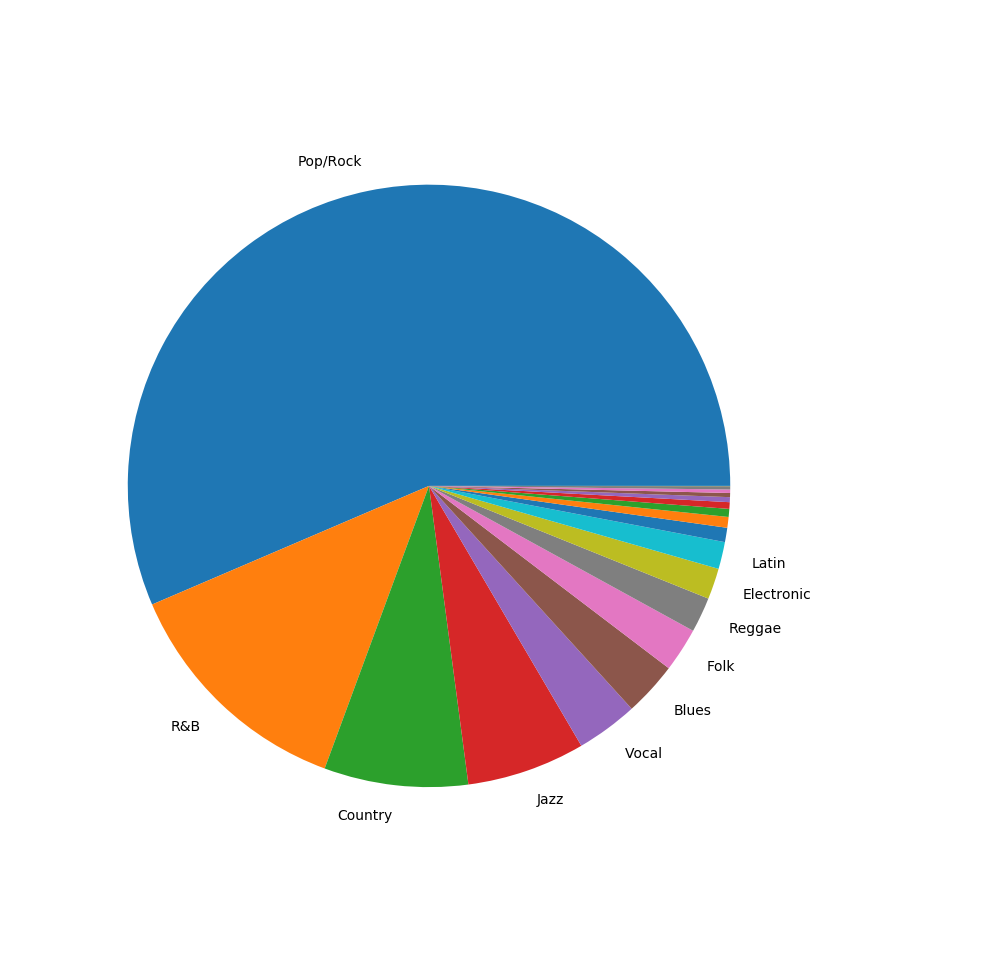
\includegraphics[width=8cm]{Figure_1.png}
\caption{The proportion of each genre}
\end{figure}
\section{Network Model to Describe the Relationship between influencers and followers}
\subsection{Basic Preparation} 
\subsubsection{Spares Graph}\quad\;
From Wikipedia, we know in mathematics, a graph with only a few edges, is a sparse graph. 
The graph density of simple graphs is defined to be the ratio of the number of edges ${|E|}$ with respect to the maximum possible edges.
For directed simple graphs, the maximum possible edges is twice that of undirected graphs to account for the directedness, so the density is:
$${\displaystyle D={\frac {|E|}{2{\binom {|V|}{2}}}}={\frac {|E|}{|V|(|V|-1)}}}$$
where E is the number of edges and V is the number of vertices in the graph. The maximum number of edges for an undirected graph is 
$${\displaystyle {\binom {|V|}{2}}=|V|(|V|-1)/2}$$ So the maximal density is 1 (for complete graphs) and the minimal density is 0.

\subsection{Directed Network of Influencers and Followers }\quad\;

We primarily concerned two ways to build the directed influential network of influencer artists and their followers: 


The first way is through the adjacency matrix, where we use rownum to represent followers' ID, and column number to represent influences' ID. Using this method we can see very directly how an artist is connected to another. And the matrix for this network mainly has two characteristics: it is extremely asymmetric and sparse. 

The reasons are easy to understand: there almost no notable mutual influences between two artists in the given data, and the total amount of artists is too large compared with the the number of influencers to a particular artist. The sparse matrix can be stored as dictionary of keys or list of lists or compressed sparse column to save space.


\begin{table}[h]
\centering
\begin{tabular}{|l|l|l|l|l|l|l|}
\hline
artist ID & 759491 & 75747 & 84053 & 74 & 66915 & 81083 \\ \hline
759491              & \      & 0     & 0     & 1  & 0     & 0     \\ \hline
75747               & 1      & \     & 0     & 0  & 0     & 0     \\ \hline
84053               & 1      & 0     & \     & 0  & 0     & 0     \\ \hline
74                  & 0      & 0     & 0     & \  & 0     & 0     \\ \hline
66915               & 0      & 0     & 0     & 0  & \     & 1     \\ \hline
81083               & 0      & 0     & 0     &    & 0     & \     \\ \hline
\end{tabular}
\end{table}
\begin{center}

In this case, we chose 5 artists from `influence\_data.csv' to build an adjacency matrix. The matrix is shown above. But of course, due to the huge size of the data, we cannot write down all of them in the thesis.
\end{center}\quad\;
The second way is to draw a directed graph to demonstrate the mutual influences of musicians from different genres.
Add different nodes that representing the artists to the network, and then connect them with arrows. \par
Due to the content length limit, we will here further illustrate the second way to establish our first model in this paper.  
To begin with, in order to take better advantage of the whole influence data set from 1930 to 2010, we (choose a thousand pieces randomly from the 42771 pieces in the given influence data, ) and use each node to represent an artist, we also assign different genres of artists with a distinct color to better distinguish them. The node's arc goes from the influencer to the follower.
We use the coding toolkit that utilizing Adjacency list to store the sparse graph to save space, and it is also convenient for us to see the influence relationship of a particular artist in this storage format. 
In this case, we can observe what are the nodes that points to a particular node (the node's in-degree) to see the amount and genres of artists that have influenced this particular artist, in the same way, by observing what nodes are a particular node pointing to, (the node's out-degree), we can gain knowledge about the amount and genres of artists that this particular artist have influenced.
We notice that different from the commonly seen directed graphs, which have at least some strong connectivities, our graph generated in this problem have almost no strong connectivities, that is to say we the influencers and the followers rarely change their positions, in fact according to our statistics, there are only 78 mutual-influence pairs in the 42770 edges and more than 5600 artists given.

The total number of outdegrees of a graph is equal with its indergees, and can be calculated with this formula:\[{O_{dt}} = \sum\limits_{i = 1}^T {{O_{di}}} \]


The total outdegrees for this graph is 42770, and the network density of the above graph is 0.0027, suggesting that the directed network of influencers and followers is a sparse graph from a mathematical perspective, for the connections,namely the edges, are to few compared with the amount of nodes.
\begin{figure}[h]
\small
\centering
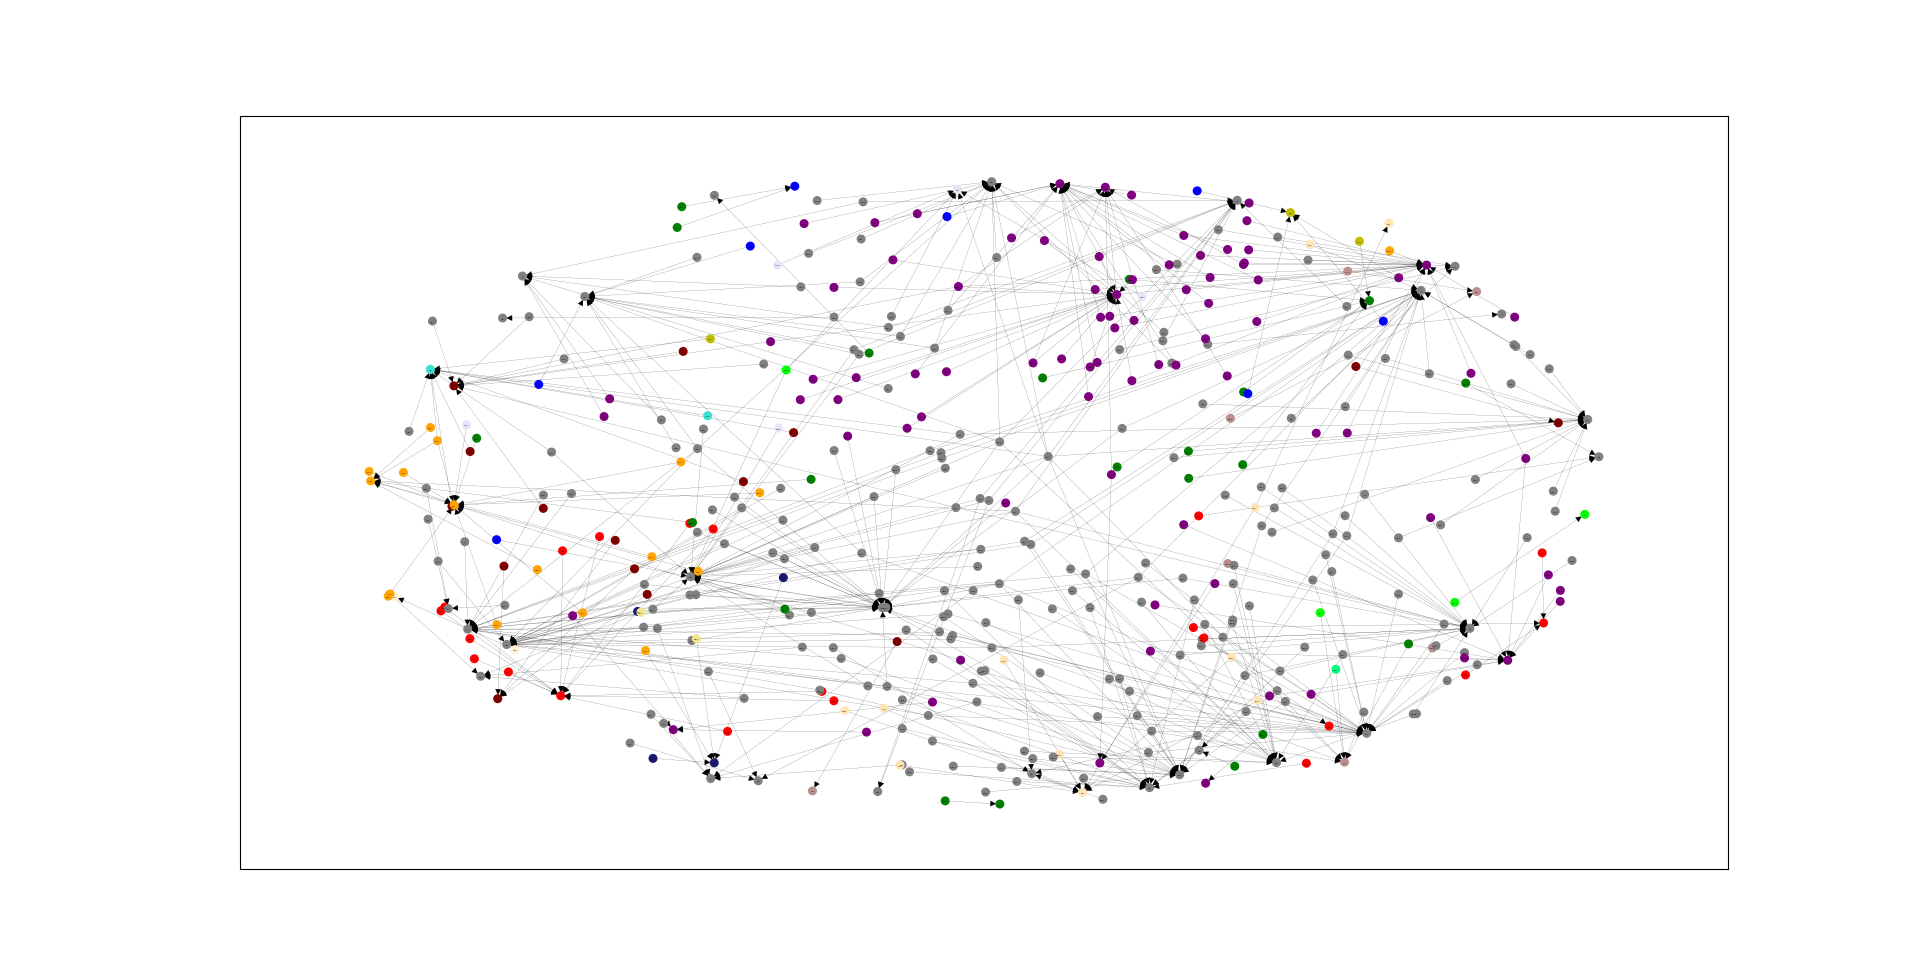
\includegraphics[width=17cm]{firstmodel.png}
\caption{network of influencer-artists and their followers}
\end{figure}

\subsubsection{Further Analysis of the First Model}\quad\;
To illustrate the first model more specifically, we can see that, generally speaking, the artist’s own genre exert more influence to him/herself than other genres.

\begin{figure}[h]
\small
\centering
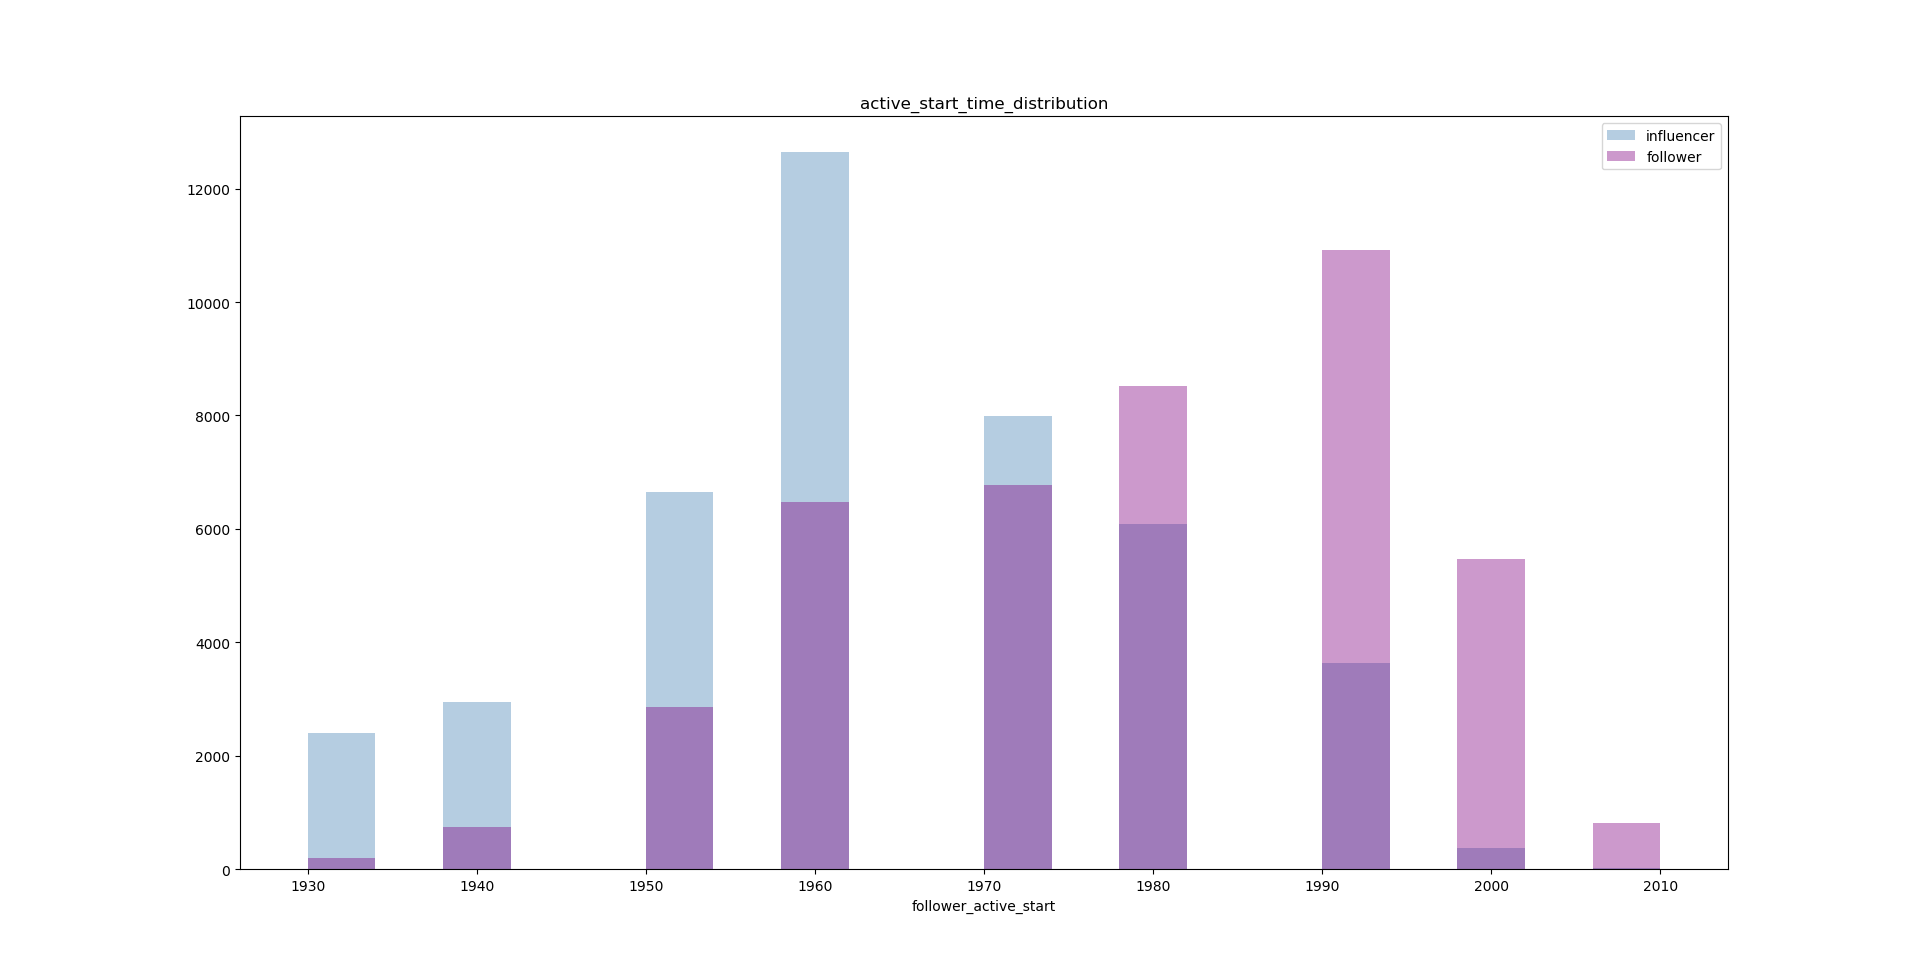
\includegraphics[width=18cm]{Figure_5.png}
\caption{active-start time of influencers and followers}
\end{figure}
We also drew a bar graph to qualitatively analyse the active-start time of influencers and followers. The height of the blue column represents the number of influencers, the height of the pink column represents the number of followers, and purple means the influencers and followers overlaps. It is clear that the influencer number obey approximately normal distribution, peaks at the year of 1960, and the follower 
number peaks at the year of 1990. In the year of 1970 and 1980, there are almost same number of influencers and followers.


\subsubsection{A 3D Model to Further Analyse The Network}\quad \;
\begin{figure}[h]
\small
\centering
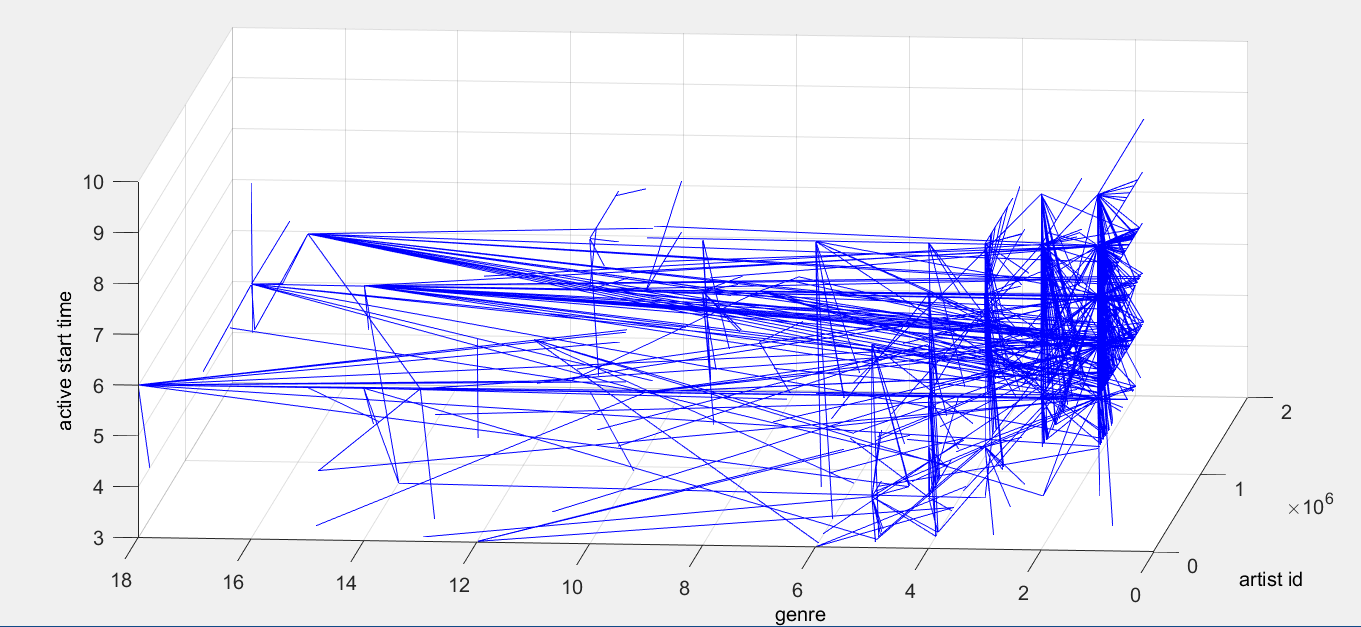
\includegraphics[width=14cm]{3D.png}
\caption{3D model of the influence\_data}
\end{figure}
In order to have a deeper understanding of the how different artists influence one another, we conducted the our second model in matlab. As shown, each of the three dimensions of the broken line graph represents genres, the year from which the artist became active and the artist\-id respectively, and each single point is to be an artist. We connected the points that have a influence relationship with each other. 
Four main conclusions are drawn from the graph:
\begin{itemize}
\item Same with the proportion pie chart in front, we can see dots are more densely packed in the right side of the graph, meaning three categories, pop/rock, R\&B and country take up most of the genres.
\item The darkest lines are the vertical lines in the right, indicating artists are more influenced by the same genre they are from, and have strong connections with the artists from the same genre. The horizontal lines are comparatively few in number, implying that the influence relationships are mainly from the artists who started to become active in different years.
\item We can see roughly from the graph that there is a downward trend for the number of Jazz genre artists, by truncating vertically versus the artist\-id axis, and upward trend for pop/rock genre artists' number as time goes.
\item We can roughly see that the ABC genre have more connections with the DEF genre, meaning the two genres are more closely related, we will cross-contrast this conclusion with the following similarity analysis among genres.
\end{itemize}



\subsubsection{Another Network from a Different Aspect}\quad \;
In a similar manner, we also depicted another directed network ignoring the genre differences of artists to demonstrate the influence relationship among artists who become be active in different years.

To do that, We assigned the artists who be active in the same year with a distinct color,no matter what genre they are from. To give an example to illustrate the graph, we made all artists who be active in 1960 as green nodes, and artists who be active in 1980 as blue nodes, we can see clearly that there is a huge amount of green nodes pointing to blue nodes ,however among the different colors of the nodes that blue nodes point to, we can hardly see any green, meaning our assumption that 'Only the artists who became active earlier can influence the latter artists' is correct on the whole. 
\begin{figure}[h]
\small
\centering
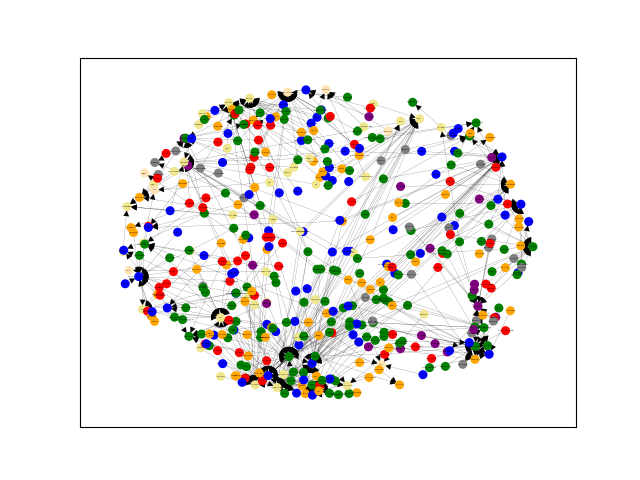
\includegraphics[width=14cm]{Figure_3.png}
\caption{influence relationship among artists of different years}
\end{figure}
\subsection{Methods to Measure `Music Influence'}
\subsubsection{Direct Way for Measuring `Music Influence'}\quad \;
As is explained above, we may use the outdegree of a node in the first model to evaluate the power of influence of that artist.
And in order to narrow the influence parameter to attain a similar effect as normalization, we use the outdegree divided by the total number of artists available. 
\[{m_d} = \frac{O_d}{T}\]\quad\;
Combining our statistics with the formula, we got the ten most influential artists, they are: \textbf{1} The Beatles, \textbf{2} Bob Dylan, \textbf{3} The Rolling Stones, \textbf{4} David Bowie, \textbf{5} Led Zeppelin, \textbf{6} Jimi Hendrix, \textbf{7} The Kinks, \textbf{8} The Beach Boys, \textbf{9} Hank Williams and \textbf{10} The Velvet Underground.
\subsubsection{Comprehensive Way for Determining `Music Influence'}\quad \;
Again making use of the connectivity of our first model, and associate it with the Dijkstra algorithm in graph theory, we developed a second way for determining 'Music Influence' as an improved plan of the first.
We divided the influence power of an artist into to aspects: his/her direct influence to others and indirect influence to others. The numerical value of direct influence is the outdegree of the node, and the indirect influence is the indirect connection of two nodes, for example, if artist A influenced artist B and artist B influenced artist C, but there is no direct connection between A and C,then we consider artist A also have influence upon artist C, in order to have a set of positive assessment criteria, we define the numerical value of indirect influence as the reciprocal of the shortest path of two nodes.
\begin{figure}[h]
\centering
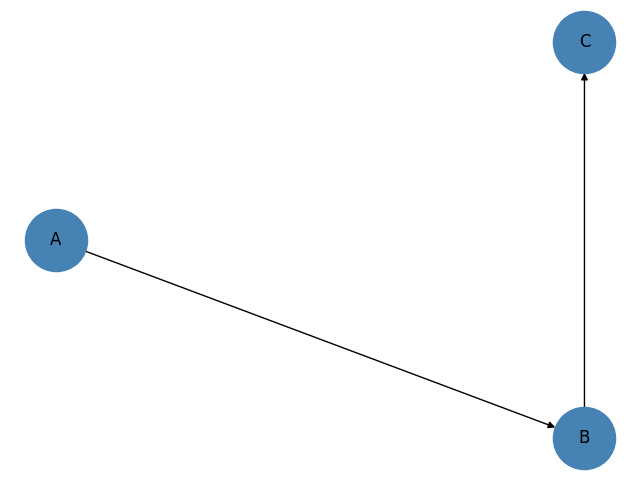
\includegraphics[width=3cm]{simple graph.png}
\end{figure}


Below is an example to demonstrate the meaning of shortest path of two nodes, there are two ways that A can be connected with C, either through A->B->C or A->D->E->C, and the shortest path is 2, the indirect influence value is 1/2.
\begin{figure}[h]
\centering
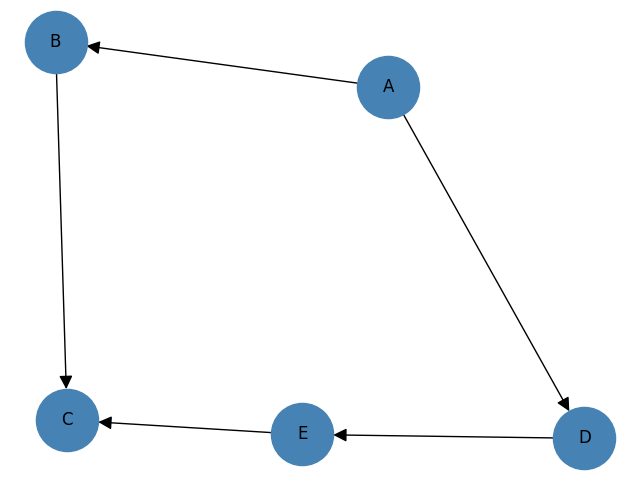
\includegraphics[width=3cm]{simple graph2.png}
\end{figure}
We then calculated all the shortest paths of each node available of the first model, take reciprocals, and added them together as the total indirect influence value of an artist. It is worth mentioning that if there isn't any path between two nodes, their path length is considered as 0 to simplify the calculation.

We defined our comprehensive evaluation parameter of node 'i' for 'music influence' as:\[{m_c} = {O_d} + \sum\limits_{i = 1}^T {(\frac{1}{{{d_i}}})} \]\quad\;
The merit of using Dijkstra algorithm to calculate the shortest paths between nodes is its considerably low complexity, which is almost linear, and Dijkstra algorithm is just fit to be applied in the calculation of sparse graphs like ours. However, it still took more than 2 hours to run the program for the comprehensive ranking of all artists, for the extremely large number of floating point arithmetic we have to do, it will only take much longer time if we use other normal methods like the Floyd algorithm. 


And the ten most influential artists calculated in this method are: \textbf{1} The Beatles, \textbf{2} Bob Dylan, \textbf{3} Chuck Berry, \textbf{4} James Brown, \textbf{5} The Rolling Stones, \textbf{6} Elvis Presley, \textbf{7} Little Richard, \textbf{8} Jimi Hendrix, \textbf{9} Muddy Waters and \textbf{10} Hank Williams.



\subsubsection{Updated Version of the Comprehensive Way for Determining `Music Influence'}\quad \;
It is noticeable that the weight of indirect influence is not very convincingly fixed, namely the decision of which is rather subjective.
From Wikipedia we know that in science, inverse-square law is any scientific law stating that a specified physical quantity is inversely proportional to the square of the distance from the source of that physical quantity. The fundamental cause for this can be understood as geometric dilution corresponding to point-source radiation into three-dimensional space.


And using this commonly mentioned formula format for reference, we intended to decrease the weight of indirect influence, and modified ${m_c}$ as:
\[{m_u} = {O_d} + \sum\limits_{i = 1}^T {\frac{1}{{d_i^2}}} \]
And using to this index calculate the 10 most influential artists out of the data, the results are:\textbf{1} The Beatles, \textbf{2} Bob Dylan, \textbf{3} The Rolling Stones, \textbf{4} Chuck Berry, \textbf{5} Elvis Presley, \textbf{6} Jimi Hendrix, \textbf{7} James Brown, \textbf{8} Little Richard, \textbf{9} Hank Williams and \textbf{10} Miles Davis.
\subsection{Simple Comparison of the Three Ranking Results}\quad \;
The three ranking results above are very close to each other, the  first two of all rankings are consistent,they are The Beatles and Bob Dylan. In general, the artists listed from the indirect method are more ``antique'' compared with the direct method, for taking the secondhand influence of an artist into consideration, the earlier artist became active the more of the following generations he is likely to indirectly influence. And ranking of the comprehensive method is kind of the compromise of the direct and indirect method, for we manually minished the weight of the indirect influence.
\section{Similarity between Genres, and between Artists}\quad\;
Below is an illustration to show the relationship between one follower and his/her influncers, we use the icon ``A9'' in the middle to represent the follower artist, as we can see, there are more than one influencer that had influenced the follower, either directly or through the connections with others. Our interest is to quantify the relationship of how many of these influencers are from the same genre as the follower, and how many are from different genres with him to see whether an artist is influenced more within the same genre or from other genres. 

\begin{figure}[h]
\centering
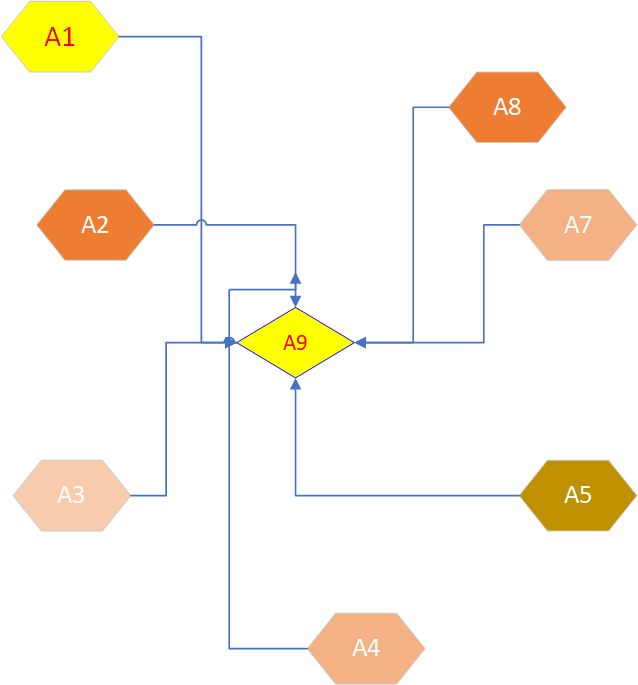
\includegraphics[width=6cm]{mind1.png}
\end{figure}





We counted the number of influnecers in the data\_by\_artists in some typical genres, and sorted all of their followers by genres.
Here is an example, we collected all the influnecers from the avant genre, and their followers' genres are shown in the next two illustrations. 

And our interpretation is: the avant genre doesn't have enough inner influences within its own genre, for more than 90\% of their followers "give up" this genre and changed their musical styles into other genres like pop/rock, electronic, new age, etc.

We can also see some connetions between avant genre and other genres. Since the majority of avant followers are pop/rock artists, we can say that avant genre is more closely related with pop/rock than with others.
\begin{figure}[h]
\centering
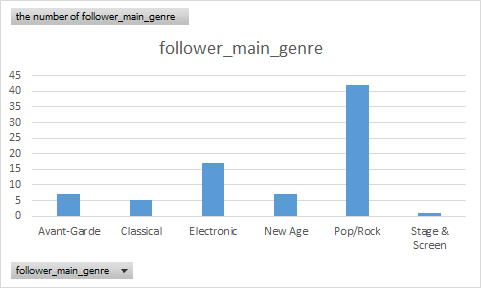
\includegraphics[width=10cm]{avant1.png}
\caption{The categories of followers by influenced by avant artists}
\end{figure}

\begin{figure}[h]
\centering
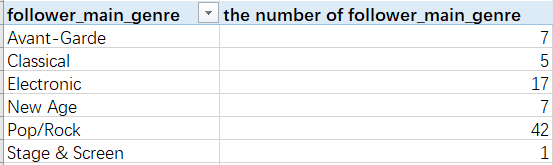
\includegraphics[width=10cm]{avant2.png}
\caption{The categories of followers influenced by avant artists}
\end{figure}

In the same way, we can say blue has a better inner influence than avant, about 30\% followers chose to stay in the same genre. And for follower artists that set foot on different paths, the majority of them also later became pop/rock artists. We can see from the statistics that blue have a closer relationship with pop/rock and R\&B than with others.
\begin{figure}[h]
\centering
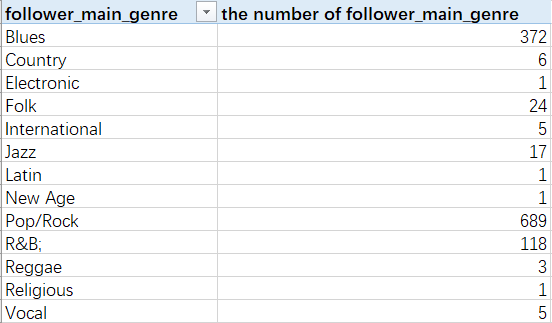
\includegraphics[width=10cm]{blue.png}
\caption{The categories of followers influenced by blue artists}
\end{figure}

Combined these two samples, we can also draw the conclusion that the pop/rock genre is a fairly ``synthetical'' genre, integrated many elements from other genres to help form their own style.

The following are results of other genres we computed.
 If we define the proportion of same-genre followers to influencers as ${p_{fi}}$, ${p_{fi}}$ can also be regarded as the ``loyalty index'' of a genre. we can also tell whether artists got more influenced by their own genre. The larger the ${p_{fi}}$, the more artists are influenced by their own genre. And we can draw the conclusion that the pop/rock genre is more self-influenced (has higher ``genre loyalty'') compared with genres like vocal and electronic.
\begin{figure}[h]
\small
\centering
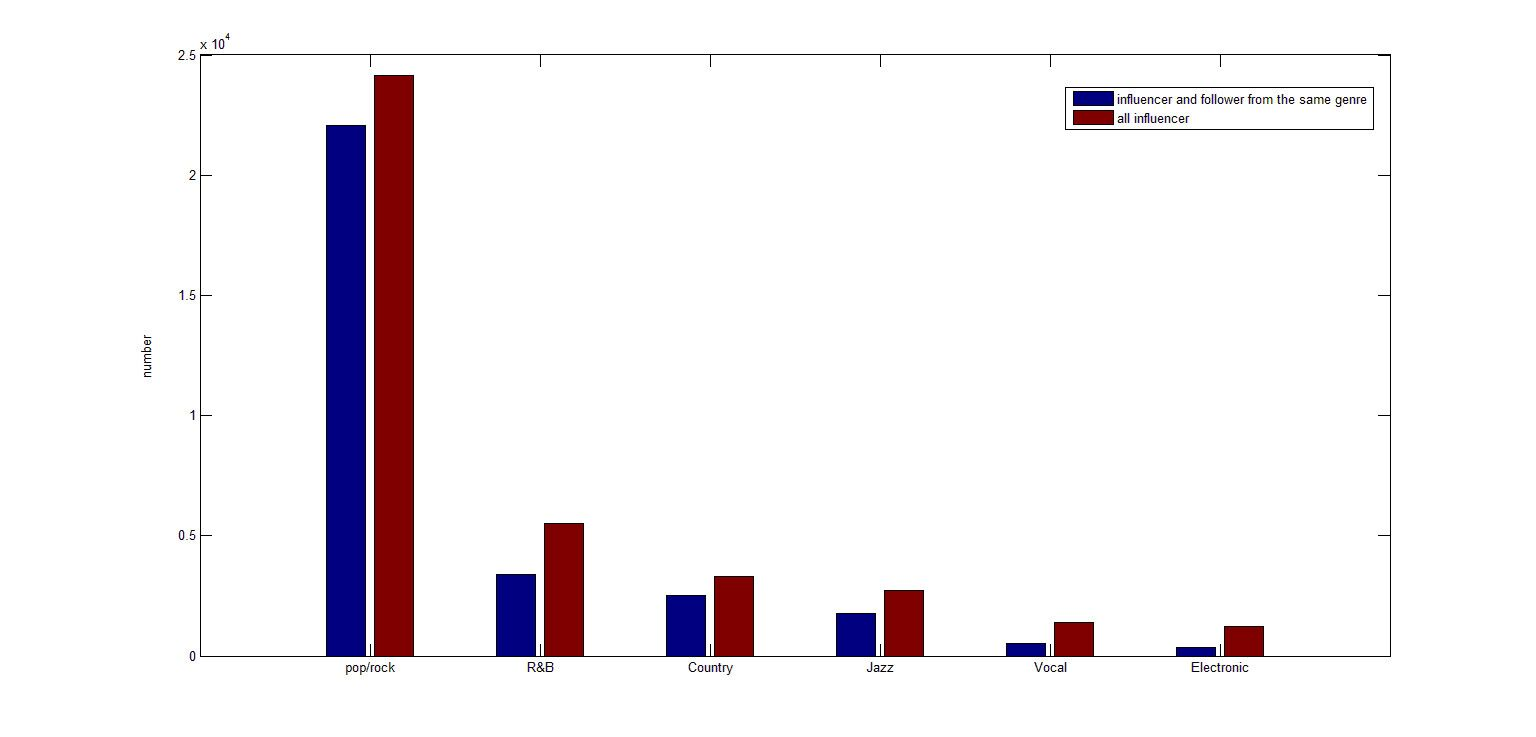
\includegraphics[width=12cm]{compareofinf.png}
\caption{Variation of Music Arguments}
\end{figure}




\begin{figure}[h]
\centering
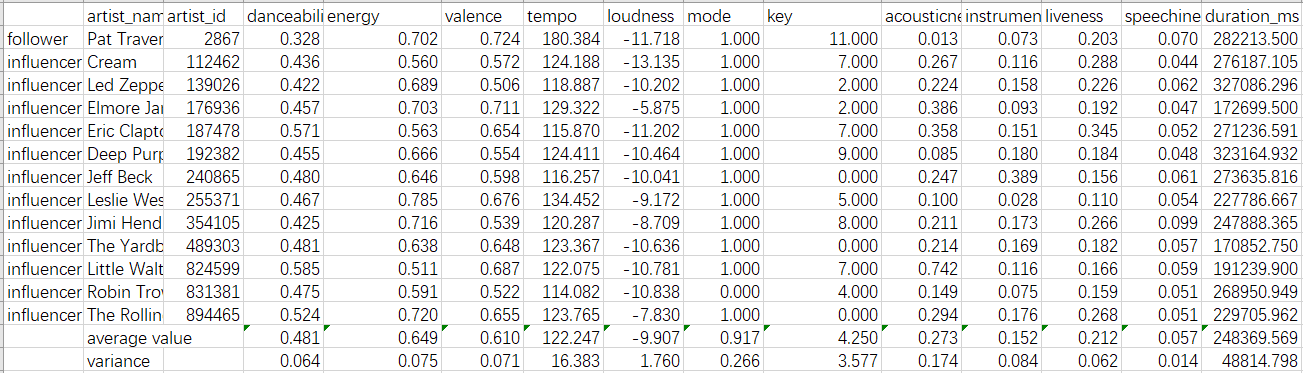
\includegraphics[width=10cm]{235.png}
\caption{Variation of Music Arguments}
\end{figure}







\subsection{Models of Similarities  }
\subsubsection{Euclidean Distance}\quad \;
In mathematics, the Euclidean distance between two points in Euclidean space is the length of a line segment between the two points. It can be calculated from the Cartesian coordinates of the points using the Pythagorean theorem.\cite{2}\par
In general, for points given by Cartesian coordinates in ${\displaystyle n}$-dimensional Euclidean space, the distance is:
$${\displaystyle d(p,q)={\sqrt {(p_{1}-q_{1})^{2}+(p_{2}-q_{2})^{2}+\cdots +(p_{i}-q_{i})^{2}+\cdots +(p_{n}-q_{n})^{2}}}.}$$



\subsubsection{General Methodology}\quad \;
We analysed the similarity among and within the genres using the data\_by\_artist database. In the data set, the music attributes of an artist are divided into 14 different aspects, take out the count (the number of songs), we consider the rest 13 different arguments of music, which are danceability(da), energy(e), valence(v)... duration(du) and popularity(p). The closer the numerical value, the more similar the two artists are in musical styles. 

We then regard the ``music space''as a 13-dimensional Euclidean space,and used the Euclidean distances of artists to describe their similarities. Refering to the Euclidean distance definition, the similarity between artists a and b can be defined as:
$${\displaystyle s_0(a,b)={\sqrt {(da_{a}-da_{b})^{2}+(e_{a}-e_{b})^{2}+\cdots +(du_{a}-du_{b})^{2}+\cdots +(p_{a}-p_{b})^{2}}}.}$$
However, the scales of different arguments also need to be taken into account. Thus we used the maximum and minimum value to normalized all the arguments before calculating the distance:
\[z_i^* = \frac{{{z_i} - {z_{i\min }}}}{{{z_{i\max }} - {z_{i\min }}}}\]
And the modified formula:
$${\displaystyle s(a,b)={\sqrt {(z_{1a}^*-z_{1b}^*)^{2}+(z_{2a}^*-z_{2b}^*)^{2}+\cdots +(z_{3a}^*-z_{3b}^*)^{2}+\cdots +(z_{13a}^*-z_{13b}^*)^{2}}}.}$$

Notice the magnitude of result is contrary to similarity, because if two artist's music styles are completely the same,the distance should be zero. 
\subsubsection{Similarity within the Same Genre}\quad \;
We began with sorting out the artists with the genres, then
each time considered the similarity of two artists (by calculating the Euclidean distance of the two artists using the above formula), and promoted that principle to every two artist within the genre and averaging all the results to get a mean value of similarity within a genre.  
Assuming a genre  ${\displaystyle x}$with ${\displaystyle n}$ artists, the similarity within this genre is:
\[S(x,x) = \frac{{\sum\limits_{j = 1}^n {\sum\limits_{i = 1}^n {s(i,j)} } }}{{n(n - 1)}}(i \ne j)\]
\subsubsection{Similarities of Different Genres}\quad \;
Assuming we want to calculate the similarity of a genre  ${\displaystyle x}$with ${\displaystyle n}$ artists and a genre  ${\displaystyle y}$with ${\displaystyle m}$ artists,
Similar with the calculation method of the prior section, the formula for calculating the similarities of different genres can be defined as:
\[S(x,y) = \frac{{\sum\limits_{j = 1}^m {\sum\limits_{i = 1}^n {s(i,j)} } }}{{mn}}\]
Also notice that the numerical pair in the calculation of one-genre similarity is order-independent, but the numerical pair in the calculation of different-genres similarity is sequential, for example the pair s(1,1) here means the similarity between the first artist from genre ${\displaystyle x}$ and the first artist from genre ${\displaystyle y}$, in the same manner the pair s(1,2) and s(2,1) have different meanings.\par
We calculated the similarities of 10 typical genres, the similarity matrix below is symmetric, so we only showed the upper triangle of it, and to make the data look more intuitionistic, we multiplied all of the actual results with 1000. The processed results are as below:
\begin{table}[h]
    \centering
    \begin{tabular}{|l|l|l|l|l|l|l|l|l|l|l|}
    \hline
        Similarity & pop & rb & country & jazz & vocal & blues & folk & reggae & elec & latin \\ \hline
        pop & 0.813 & 0.808 & 0.712 & 0.884 & 0.867 & 0.864 & 0.885 & 0.877 & 1.021 & 0.868 \\ \hline
        rb &  & 0.810 & 0.703 & 0.846 & 0.892 & 0.842 & 0.885 & 0.858 & 1.024 & 0.816 \\ \hline
        country &  &  & 0.605 & 0.745 & 0.738 & 0.744 & 0.853 & 0.806 & 1.004 & 0.738 \\ \hline
        jazz &  &  &  & 0.743 & 0.791 & 0.843 & 0.786 & 0.995 & 1.115 & 0.864 \\ \hline
        vocal &  &  &  &  & 0.620 & 0.845 & 0.676 & 1.078 & 1.231 & 0.894 \\ \hline
        blues &  &  &  &  &  & 0.845 & 0.845 & 0.925 & 1.103 & 0.858 \\ \hline
        folk &  &  &  &  &  &  & 0.729 & 1.026 & 1.189 & 0.885 \\ \hline
        reggae &  &  &  &  &  &  &  & 0.855 & 1.030 & 0.891 \\ \hline
        elec &  &  &  &  &  &  &  &  & 1.057 & 1.069 \\ \hline
        latin &  &  &  &  &  &  &  &  &  & 0.870 \\ \hline
    \end{tabular}
\end{table}

\textbf{The similarity matrix is the most important conclusion in the whole paper.} \\

It contains tremendous information in the similarity among different genres and within one genre.  
If space allows it, we can dozens of subconclusions from the matrix.
Here we only list five examples for reference: 
\begin{itemize}
\item The genre with the largest inner similarity is country, meaning the feature of country style music is with the brightest characteristics and easiest for people to distinguish.
%具体音乐特征回头要写
\item The genre with diminutive cross-genre similarities(shown with rather large values in matrix) like the electronic music, also suggests that its a rather distinct style from others.
\item Genres with larger cross-genre similarities than inner similarities, like Latin music's inner similarity is smaller than with R\&B, imply that people may be hard to tell Latin music from R\&B music and vice versa. 
\item The similarities of pop/rock with others and with itself are all quite close. As we have mentioned in the preceding section, this data better explained that pop/rock music is likely to be a combination and derivative of all other previously existing genres.
\item The inner similarities are larger cross-genre similarities in general.
\end{itemize}

For purpose of better visualizing data of similarity matrix, we also drew a thermodynamic chart in below. The genres with lower similarities have a color toward red trend.
Note that the graph is also symmetric Because of the attributes of similarity matrix. 
The color of the downward sloping diagonal is lighter (tends to be in blue series), means inner similarities are more significant. Also the row and column which represent electronic music has the darker color, in agreement with the conclusion mentioned above. 

 \begin{figure}[h]
\centering
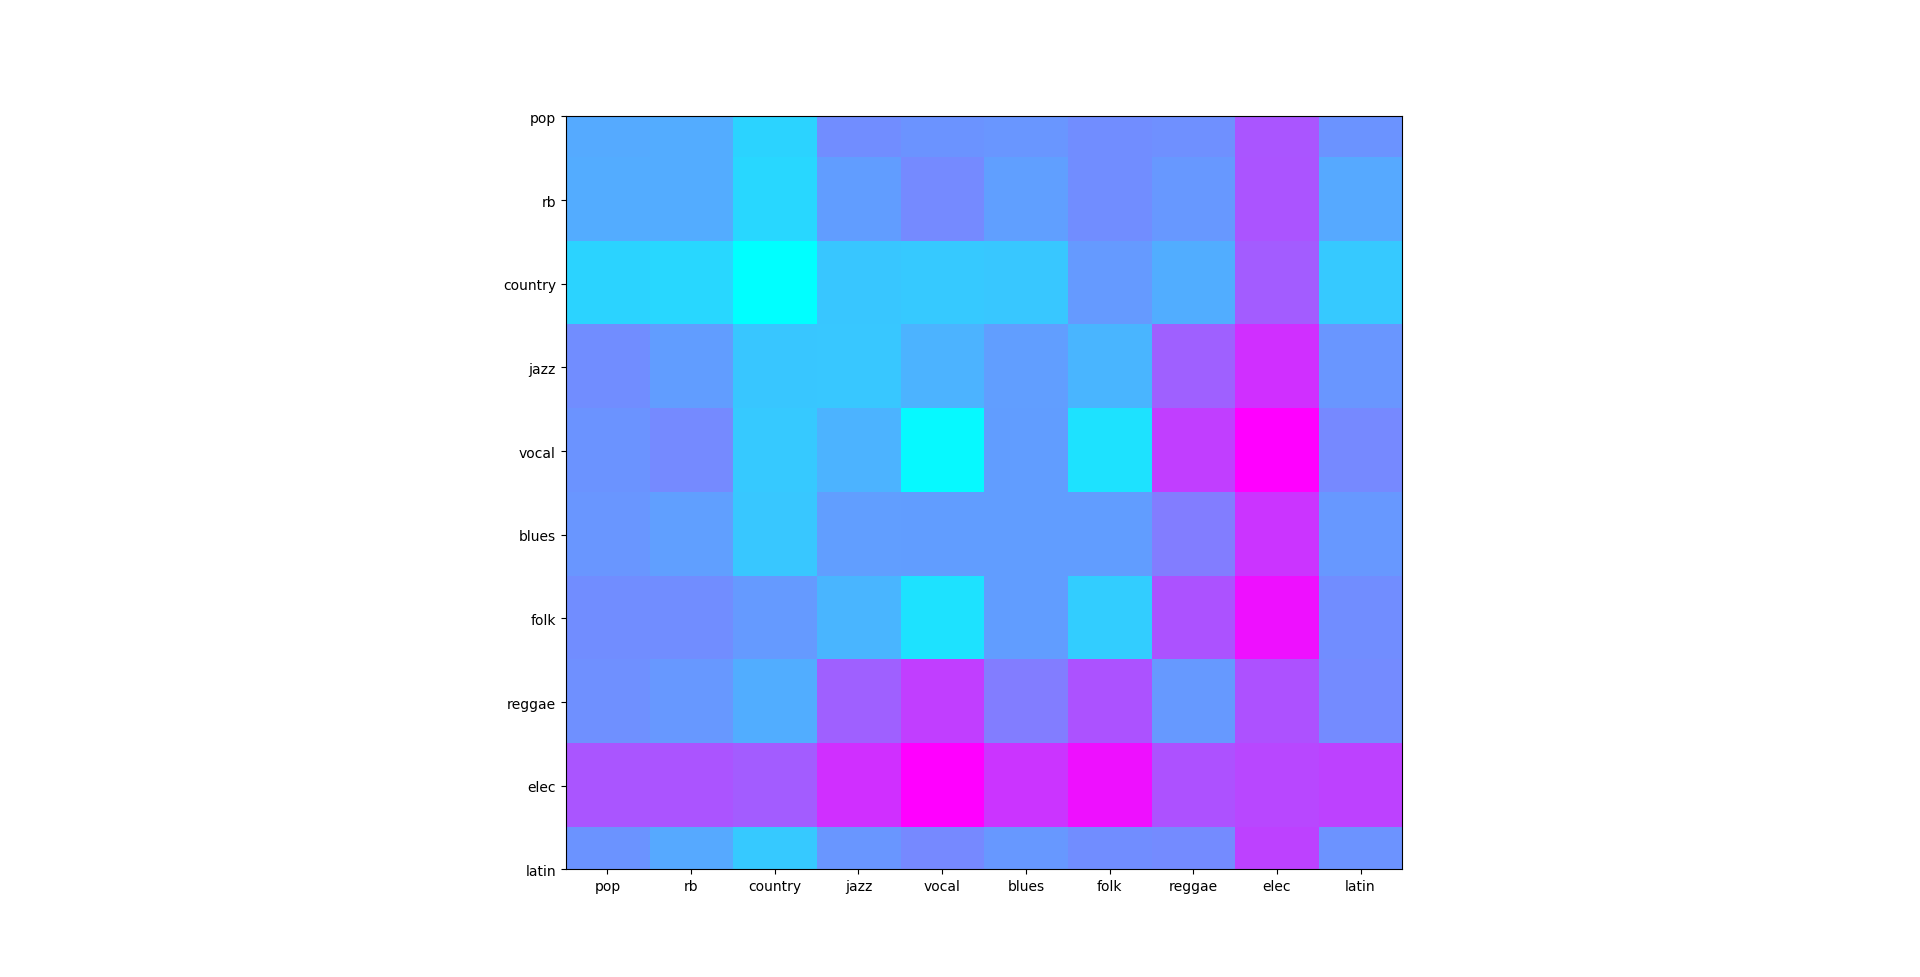
\includegraphics[width=12cm]{thermodynamic chart.png}
\caption{thermodynamic chart}
\end{figure}



\subsection{A Supplementary Methodology to Measure Similarity}\quad \;
\subsubsection{Pearson Correlation Coefficient}
Pearson's correlation coefficient is the covariance of the two variables divided by the product of their standard deviations:\cite{3}
$${\displaystyle \rho _{X,Y}={\frac {\operatorname {\mathbb {E} } [(X-\mu _{X})(Y-\mu _{Y})]}{\sigma _{X}\sigma _{Y}}}}$$
where:
${\displaystyle {\sigma _{X}}}$ and ${\displaystyle {\sigma _{Y}}}$ are standard deviations of ${\displaystyle X}$ and ${\displaystyle Y}$\\
${\displaystyle \mu _{X}}$ and $\mu _{Y}$ are the means of ${\displaystyle X}$ and ${\displaystyle Y}$\\
${\displaystyle \operatorname {\mathbb {E} }}$ is the expectation.\\
In a sample, the Pearson correlation coefficient is commonly represented by ${\displaystyle r_{xy}}$. Given paired data ${\displaystyle \left\{(x_{1},y_{1}),\ldots ,(x_{n},y_{n})\right\}}$ , ${\displaystyle r_{xy}}$ can be calculated as:
$${\displaystyle r_{xy}={\frac {n\sum x_{i}y_{i}-\sum x_{i}\sum y_{i}}{{\sqrt {n\sum x_{i}^{2}-(\sum x_{i})^{2}}}~{\sqrt {n\sum y_{i}^{2}-(\sum y_{i})^{2}}}}}.}$$
Different from the Euclidean distance, the correlation coefficient is a positive index for measuring similarity.

We then attempted to calculate the correlation coefficient of each two artists as a supplementary to better testify the result from our first method. However, the results are not very desired, for the results came very near each other.


\subsection{The Practical Influence of the Alleged Influencers to Followers}\quad\;
We selected ten followers randomly, and then studied the consistencies of music arguments between a follower and all of his direct influencers. First we calculated the Euclidean distance and found them rather lower than truly random artists. We found that the similarity between influencer and followers are higher the normal situations. For example, PJ Harvey's distance to his influencers average by 0.640 which is significantly lower than other than the distance between two randomly selected artists-but we should aware that most of his influencers and himself is from the same genre. And then by calculating the average value of arguments of the influencers, and compare the corresponding values of the follower, we researched to what extent a follower is practically affected by his alleged influencers. 

As our example below shows, the arguments’ mean value from the influencers are close with those of the follower, also by calculation (using the Euclidean distance mentioned), we found that the similarity among one follower and his/her influencers are more apparent than  with  similarity between the follower and random artists in his/her genre. So we can say the alleged influencers do have a practical influence upon the follower.

We also computed the variance of all influencers and the follower, and found them to be fluctuating in an acceptable range, what is also noteworthy is that the arguments of ``tempo'' and ``loudness'' are extraordinarily small in relative size. Therefore, we consider these two characteristics of music to be more ``\textbf{contagious}'', for these two aspects exert a much deeper and firmer influence on an artist than other characteristics.\par
We suggest that the mean value of these features of influencers is just fitted to the same feature of the follower. We tried to use hypothesis test. But we cannot confirm the distribution is normal. It is a pity.

\subsection{Distinct Characteristics of Genres}\quad\;
We normalized the 13 music arguments, and calculated the mean values of which in the typical genres to determine the distinct Characteristics of genres.
Here are some interesting results:

\begin{itemize}
\item The features of electronic music are most prominent, with high values in danceability(0.6), energy(0.6) and instrumentness.\\
\item The features of pop/rock are high popularity and energy(0.6).\\
\item  The feature of Latin is high valence(0.64).\\
\item The feature of folk is low energy(0.3).\\
\end{itemize}
\section{Variation Tendency of Genres Through Time}
\subsection{The Change in Numbers of Artists in a Genre}
\begin{figure}[h]
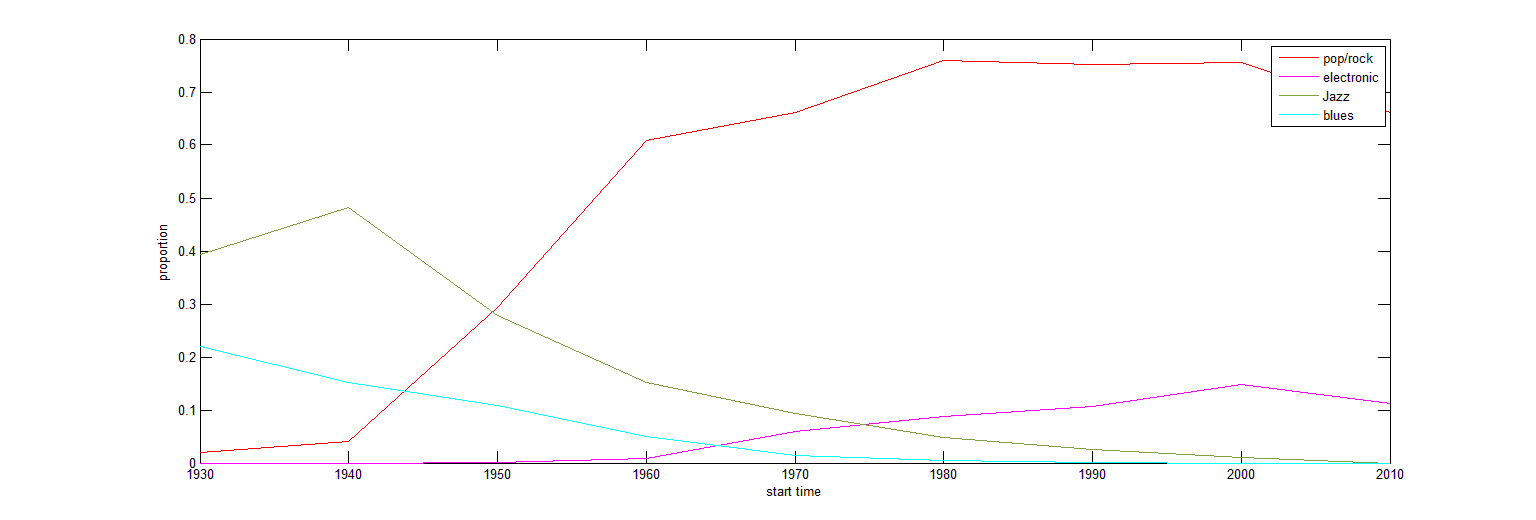
\includegraphics[width=13cm]{4genre.png}
\caption{Variation in Number of Artists}
\end{figure}

we picked a few typical genres to study as depicted in the illustration above.

%注意!背后蕴含的文化原因琛哥如果想写就写写吧,我没时间了解这方面。
\begin{itemize}
\item \textbf{Pop/Rock:}\\
As we can see the pop/rock genre grew explosively in the last century, especially from about 1940 to about 1960, multiplied almost 14 times in its relative size with other genres.
\item \textbf{Electronic:}\\
The electronic genre is rather a newly-developed genre, started to emerge as late as in 1960, but is only about one seventh to the size of pop/rock.
\item \textbf{Jazz:}\\
Jazz music reached its top in reached its summit in proportion in around 1940, and has begun to fade out since then.  
\item \textbf{Blue:}\\
The blues has been seceding out of the stage of music world for almost a century, and has a tendency to become only a memory in the history.
\end{itemize}



\subsection{The Implying Factors in the Changing of Music Styles}\quad\;
From the line chart below we can see the overall trend of different music features. And in the following sections,
 we will explain the variance and tendency about different features. To calculate the change, we used \textbf{difference method}
$$D_{i}=\frac{F_{n_i}-F_{n_{i-1}}}{1}$$
After the quantization by using the difference method, we can verify the conclusion that we seen in the chart.
\begin{itemize}
\item Energy
\end{itemize}\quad\;
From the line chart, we can know that the throughout the whole $20^{th}$ century, the energy in the music is going up.
Furthermore, we find out that in the age of $1960s$, the increase of energy in the music is bigger. We assume that it is 
strongly connected to the society and culture in those days.\par
We know that 1960s is age of rebellion and hippies. They always tend to shout out their opinions and they 
are never afraid to fight against the government. In the mean time, rock music, as a unique genre, is coming
to the main stream of the music world. The rebellious spirit become the catalyst of music. In return, music can
 sensitize people and make them aware of important events and take actions.\cite{4} Therefore, the energetic music become 
more and more popular. Music in this era encourages people to fight for themselves and resist the injustice.
Only with energy can people be inspired.
\begin{itemize}
\item Acousticness
\end{itemize}\quad\;
In the old time, classical music focus on melody and timbre. People go to concert to enjoy themselves. However,
nowadays musicians compose songs mainly to express themselves. The situation started in 1960s, exactly at the 
same time, we find that the feature `acousticness' is declining. We know that classical music is known for its
beautiful melody and people always immerse themselves in it. But classical music is becoming less popular 
in modern time. In the contrary, the rising genre of music world-pop\&rock is not that acoustic. To some people,
it is even regarded as noise. After all, it is just about the change of people's taste.
\begin{itemize}
\item Speechiness
\end{itemize}\quad\;
In the data-by-year table, we also find out that compared to the age of 1950s and 1960s, the index of speechiness
of 1970s is higher. We assume that it is concerned with the born of rap.  A famous comedian Rudy Ray Moore, recorded his
comedy in a fast-speaking tone.\cite{5} His career come to the prime 
in 1960s. Then his recordings and comedies become popular and wide-accepted, it derived into rap. And Rudy
Ray Moore himself became the ``Godfather of Rap''. Meanwhile, in the african american community in Bronx,New York,developed rap in the
 strict sense.Since the rap becomes popular as a music genre. No wonder the speechiness of music is getting higher in 1970s.
\begin{itemize}
\item Popularity
\end{itemize}\quad\;
\begin{figure}[h]
\centering
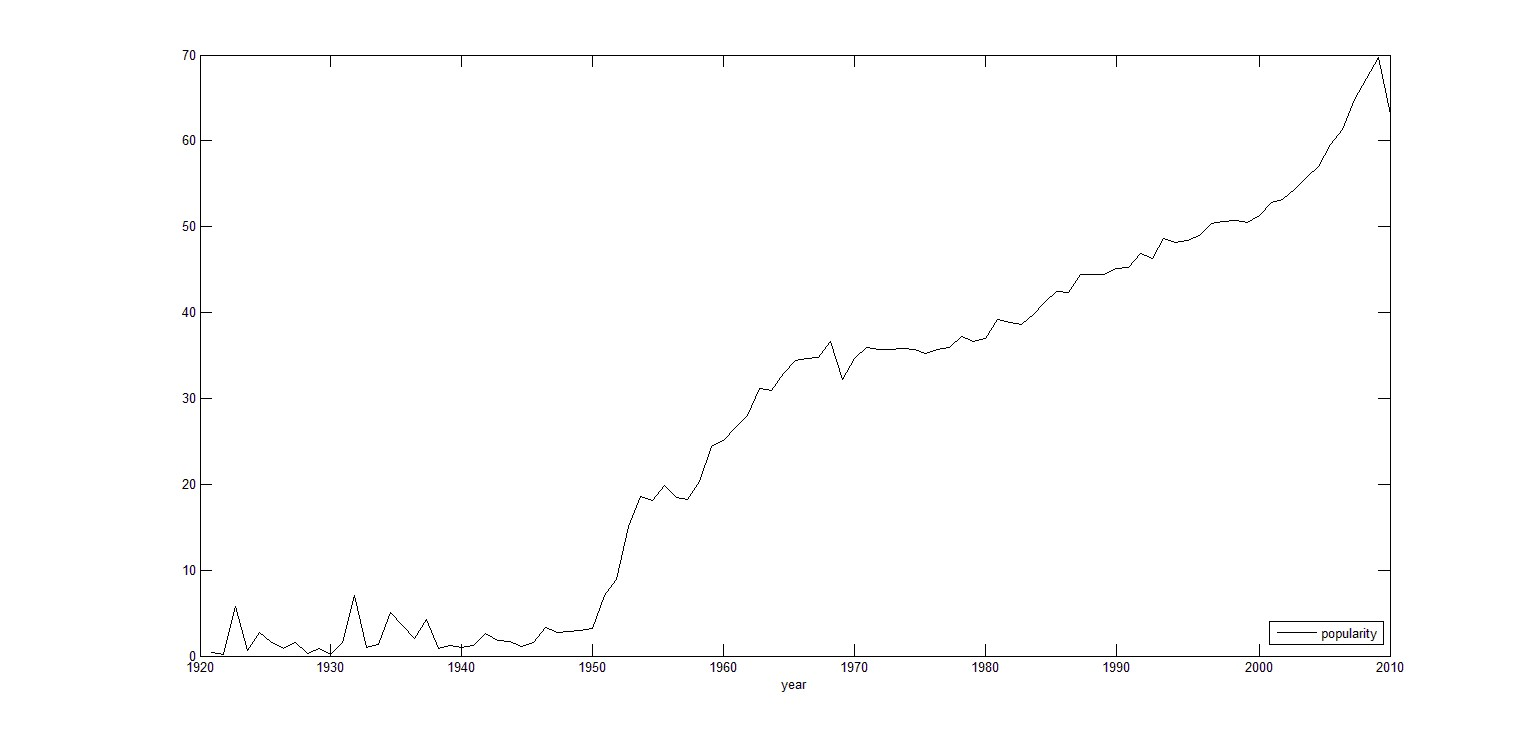
\includegraphics[width=12cm]{popular.png}
\caption{Variation of popularity}
\end{figure}

From the line chart we can directly know that the popularity of music is increasing significantly throughout the time.
It is so obvious that we don't even need to calculate the difference. We suggest that it is due to the increase of the quality 
of life. With the increase of productivity, people are living a happier life. While people are having more spare time, they must find something to fulfil themselves. 
Also, after people get satisfied in material life, they always tend to find their pleasure in spiritual life. Without doubt, music is an indispensable part
 of spiritual world. Therefore, people listen to music more often. In this case, the popularity of music rises. \par
Besides, we hold the view that the innovation of technology can also affect the increase of popularity. From the chart we can see that in 2000s the popularity  increased significantly. 
First, the Internet gives a huge help in spreading music. We listen to music in our app everyday, it's hard to imagine for us that how would we enjoy music without Internet. Secondly, 
electronic device is a big help to music. With modern recording devices and electronic instruments, artists can compose their songs more easily. And with the aid of newest headphones, people
can enjoy the best music wherever they are. Technologies definitely helped us better enjoy music and made us more like music.

\begin{figure}[h]
\small
\centering
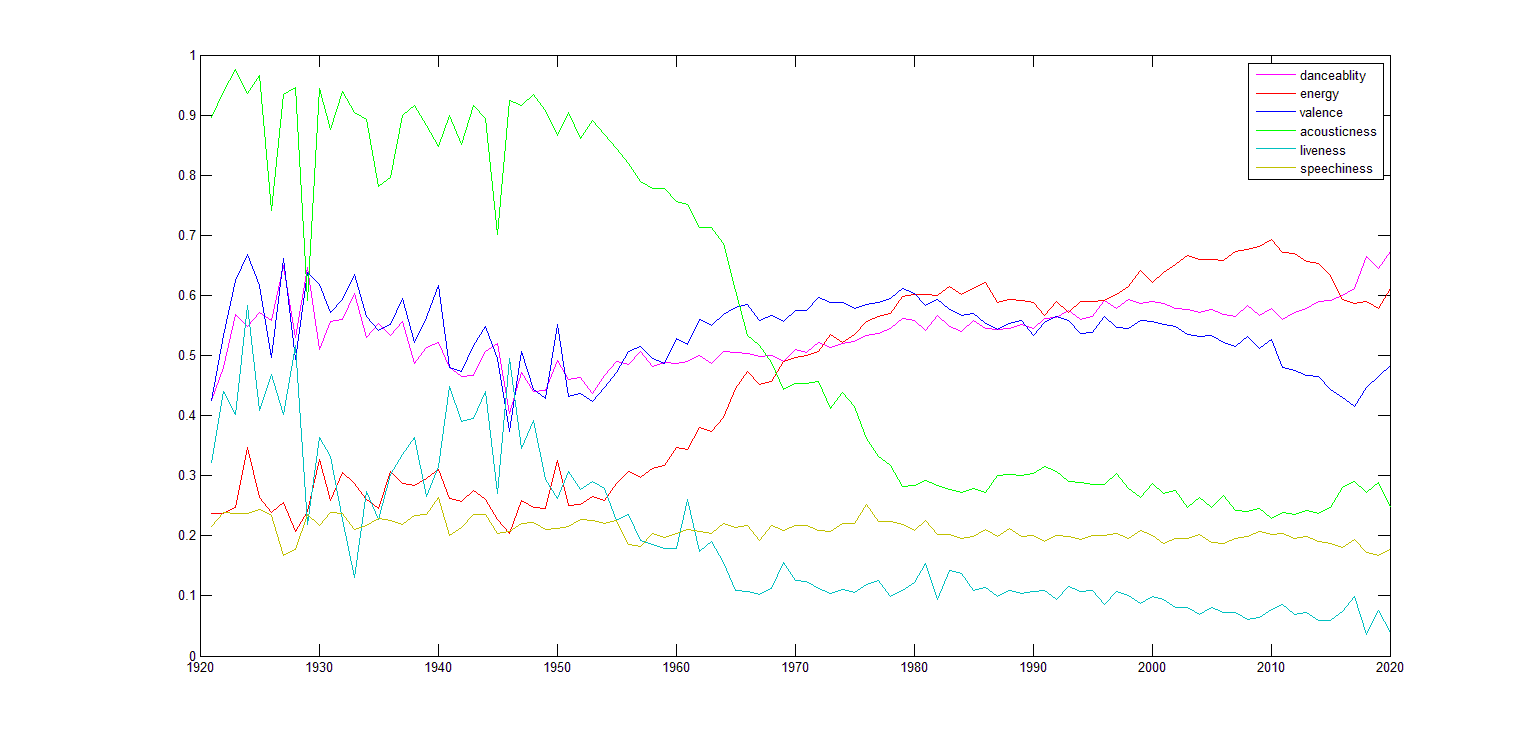
\includegraphics[width=12cm]{numbertrend.png}
\caption{Variation of Music Arguments}
\end{figure}


\section{Indicators for Revolutions in Musical Evolution}
\subsection{Music Arguments Indicators}
We can also harness the iconograph above to estimate possible arguments implying musical revolutions, which are the eras that music features turned sharply, as shown, it is about the 1950s and 1960s. And the arguments indicators are mainly acousticness, liveness and energy for the magnitudes of the changes are very arresting in these features. Just as we claimed in the previous section. What we seen in the graph has also been proved by calculating the difference.


\subsection{Indicators for Dynamic Influencers}\quad\;
In this section, in order to simplify the model, we presume the ``popularity'' attribute in data\_ by\_ artists manifests the quantitative value for ``dynamical influence''. 

To decide indicators for dynamic influencers, we first selected the top 100 
artists with highest popularity attribute. And after kicking out those who are not influencers in the influence\_data, there are still 99 artists left. We calculated the average values of their rest 12 musical arguments (count not included).
Next we picked 498 followers, and calculated the average values of musical arguments of them.

And we can conclude that in general,artists whose music have higher values of acousticness, instrumentalness, duration, lower energy, key and speechiness,etc, are more likely to become ``dynamic influencers''.


\subsection{Great Artists as revolutionists}\quad\;
As we already knew that 1950s and 1960s is the age of ``music revolution''. We find some artists from 1950s and 1960s who is most influtial in our network: the Rolling Stone, Chuck Berry and Elvis Presley.\par
We analysed their music features. Among all of the artists at the same age, their popularity is significantly higher. Specially, Chuck Berry's music has higher tempo. And both rolling stone and Chuck Berry's songs has more energy. Because we already knew that the rising of energy and tempo is the feature of the age and they are the most influential artists of all time. To some extend, we can say they are leading the age. They are the leader of the music.









\section{Integral Evaluation of Strengths, Weaknesses and Conclusions}
\begin{large}
\textbf{Strength}
\end{large}
\begin{itemize}
\item We make fully use of the influence data and make it into a influence-following network. The evaluation method 
can precisely measure the influence of different artists. We didn't just find the adjacent node. However, we take indirect
influence into consideration. Thus the evaluation result of the network is satisfying. The highly ranked influencer is 
 also famous and known to us all.
\end{itemize}
\begin{itemize}
\item We combined the data and trend with the background of the era. There are revolutionary moment of music
 in the history. And from the time of the change, we can look back into the history. The social event and the people's status of life ata that
time is concerned to the change of music.
\end{itemize}
\begin{itemize}
\item Due to the large quantity of indicators of music. It's hard to find a way to evaluate the similarity between genres and artists.
 The statistic tool we utilized can take all of the indicators into consideration and evaluate them in a comprehensive way.
\end{itemize}
\begin{large}
\textbf{Weakness}
\end{large}
\begin{itemize}
\item Our model is totally based on the data that the problem provided. In this case, our model's robustness is highly relied on
the accuracy of the dataset. Therefore, if the data is not reliable, our conclusion cannot be assured.
\end{itemize}
\begin{itemize}
\item We do not know that whether the value of different features obey normal distribution or not. If the value is normal distributed, we can utilize \textit{hypothesis test} to test if follower's feature is fit to the influencer's feature. Hypothesis test is a more logical tool, but it's a
pity that we can't confirm the data fits normal distribution. So what we could do is just calculate the variance of the data and compare the feature
of follower with the mean value of the feature of influencers.
\end{itemize}
\begin{center}\textbf{A Document to ICM Society}
\end{center}
\section{A Letter To ICM}\quad\
Dear ICM Society:\par
As an inalienable part of human society, music is not only for entertaining people, but also plays an important role in the process of human society development. According to your request and the data you provided us, our team has completed the model to measure the influence of music, and explored the trend of evolution and revolution of musicians and genres. \par
First of all, in order to determine the music influence of artists, the network reflecting the relationship between influencer artists and followers artists is constructed. By analysing the network, we find some of the greatest artist who is most influential. They are indispensable in music history. In order to show the music leader of time, we also built influence networks at different ages.\par
Secondly, in order to measure the influence of different artists, through correlation analysis, this paper analyzes the similarity within one and between different genres according to the music characteristics of different artists. The results show that the correlation coefficient of country within the genres is the largest, that is, the music characteristics of artists within the genres are relatively similar, and the degree of mutual influence is large. From the perspective of inter genre analysis, vocal has a high degree of correlation with other genres, which indicates that this genre has a high proportion of reference from other genres, and reflects the cooperation and learning of artists among the genres.\par
In the result we calculated, we found several influential features have undergone great changes in the 1950s and 1960s. \par
Influenced by the impact of war, cultural changes and the emergence of new technologies, American music is constantly evolving. The trend of music is changing from classical music to secular music. At the same time, new elements of music from other countries are absorbed to realize the international development of music.\par
Music, as the crystal of human wisdom, is a sign of the evolution of human civilization. After making the living is no longer the problem for humans, we start pursuing the peace and satisfaction of our spirit. As we all know, human’s desire can never be satisfied, we all desire the better quality of life after we satisfy the older one. So in order to achieve the real happiness of life, The only way for us is to improve the level of our spirit through the graceful music. In such case, music is of vital importance for individual happiness. \par
The model we built is totally based on your given data. However, if we want to add some new music genres or song characteristics, our models and conclusions is going to be change. When establishing the influence model, we selected several important musical characteristics for similarity analysis. If the newly given data includes some very representative features. We can add it into the calculation of network influential. Also, our analysis of music development is based on existing data and genre popularity and characteristics. If the new data has a greater impact on the current proportion of genre popularity over the years, then our conclusions will have to be changed significantly. \par
Good music in a rightful place makes people fit in the atmosphere more easily.
\begin{flushright}
Sincerely yours,

Team 2100545
\end{flushright}
\begin{thebibliography}{99}
\bibitem{1}Four datasets given with the problem.
\bibitem{2}wikipedia.org Euclidean\_distance
\bibitem{3}wikipedia.org Pearson\_correlation\_coefficient
\bibitem{4}
Music as a cultural context for change : a study of Rock Music of the 1950s and 60s.Sarah Toraason
\bibitem{5}wikipedia.org Rudy\_Ray\_Moore
%%%%%%%%%%%%%%%%%%%%%%%%%%%%%%
\end{thebibliography}
\section*{Appendix}

\textbf{python codeto build network}\\
 import pandas as pd\\
from pandas import DataFrame\\
import matplotlib.pyplot as plt\\
data=pd.read\_csv("influence\_data.csv",header=None)\\
import networkx as nx\\
import numpy as np\\
data2=data.drop([0])\\
dict1={}\\
G2 = nx.DiGraph()\\
for i,r in data2.iterrows():\\
\quad    G2.add\_node(r[0])\\
\quad    G2.add\_node(r[4])\\
\quad    G2.add\_edge(r[0],r[4],weight=0.01)\\
\textbf{python code to calculate distance and similarity}\\
from sklearn.preprocessing import MinMaxScaler\\
mm=MinMaxScaler()\\
data.iloc[:, 2:14] = mm.fit\_transform(data.iloc[:, 2:14])\\
dis=[]\\
import numpy as np\\
for i in range(80):\\
    for j in range(80):\\
        ja.append(np.linalg.norm(np.array(ele.iloc[i,1:11]).astype(float)-np.array(la.iloc[j,1:11]).astype(float)))\\
print(np.mean(ja))\\
\textbf{python code to calculate the influence of artists}\\
for i in G2.nodes():\\
    a=0.0\\
    for j in G2.nodes():\\
        if(i!=j and nx.has\_path(G2,i,j)):\\
            a+=1/nx.shortest\_path\_length(G2, source=i, target=j)**2\\
    dict1[i]=a\\
dict1=sorted(dict1.items(),key = lambda kv:(kv[1]),reverse=True)\\
print(dict1)\\


\textbf{python code to sort data}\\
ax=-1\\
w=True\\
for i,r in datareg.iterrows():\\
    ax+=1\\
    w=False;\\
    for i1,r1 in datare.iterrows():\\
        if(r1[0]==r[0]):\\
            w=True\\
            break;\\
    if(w==False):\\
        datareg.drop(index=ax,inplace=True)\\
\end{document}
